\documentclass[conference]{IEEEtran}
\IEEEoverridecommandlockouts

\usepackage{cite}
\usepackage{amsmath,amssymb,amsfonts}
\usepackage{algorithmic}
\usepackage{graphicx}
\usepackage{textcomp}
\usepackage{xcolor}
\usepackage{csvsimple}
\usepackage{rotating}
\usepackage{subfig}
\usepackage{float}
\usepackage[toc,page]{appendix}
\usepackage{url}
\usepackage[capposition=top]{floatrow}
\usepackage[skip=8pt,font=scriptsize]{caption}

\usepackage{listings}
\usepackage{color}

\definecolor{dkgreen}{rgb}{0,0.6,0}
\definecolor{gray}{rgb}{0.5,0.5,0.5}
\definecolor{mauve}{rgb}{0.58,0,0.82}

\lstset{frame=tb,
	language=Java,
	aboveskip=3mm,
	belowskip=3mm,
	showstringspaces=false,
	columns=flexible,
	basicstyle={\small\ttfamily},
	numbers=none,
	numberstyle=\tiny\color{gray},
	keywordstyle=\color{blue},
	commentstyle=\color{dkgreen},
	stringstyle=\color{mauve},
	breaklines=true,
	breakatwhitespace=true,
	tabsize=3
}

\usepackage{wrapfig}
\usepackage{lscape}
\usepackage{rotating}
\usepackage{epstopdf}
\usepackage{array}
\usepackage{makecell}
\renewcommand\theadalign{bc}
\renewcommand\theadfont{\bfseries}
\renewcommand\theadgape{\Gape[4pt]}
\renewcommand\cellgape{\Gape[4pt]}


\definecolor{codegreen}{rgb}{0,0.6,0}
\definecolor{codegray}{rgb}{0.5,0.5,0.5}
\definecolor{codepurple}{rgb}{0.58,0,0.82}
\definecolor{backcolour}{rgb}{0.95,0.95,0.92}

\lstdefinestyle{mystyle}{
	backgroundcolor=\color{backcolour},   
	commentstyle=\color{codegreen},
	keywordstyle=\color{magenta},
	numberstyle=\tiny\color{codegray},
	stringstyle=\color{codepurple},
	basicstyle=\ttfamily\footnotesize,
	breakatwhitespace=false,         
	breaklines=true,                 
	captionpos=b,                    
	keepspaces=true,                 
	numbers=left,                    
	numbersep=5pt,                  
	showspaces=false,                
	showstringspaces=false,
	showtabs=false,                  
	tabsize=2
}

\lstset{style=mystyle}

\def\BibTeX{{\rm B\kern-.05em{\sc i\kern-.025em b}\kern-.08em
		T\kern-.1667em\lower.7ex\hbox{E}\kern-.125em}}
\graphicspath{ {fig/} }


\begin{document}
	
	\title{Simulation and Analysis of Wireless Sensor Network using Message Passing Interface }
	
	\author{
		\IEEEauthorblockN{Samarasekara Vitharana Gamage, Bhanuka Manesha}
		\IEEEauthorblockA{	bsam0002@student.monash.edu \\28993373}
		\IEEEauthorblockA{\textit{School of Information Technology} \\
			\textit{Monash University}\\
			Malaysia}
		}
	\maketitle
	
	\begin{abstract}
		Phasellus ut venenatis ante. Nullam faucibus felis nec neque laoreet, sed luctus nulla gravida. Phasellus velit tellus, semper id viverra vitae, semper sit amet lorem. Nam congue efficitur tristique. Aliquam bibendum enim mattis nulla pellentesque venenatis. Vivamus varius, arcu id ultricies porttitor, dui arcu pretium est, et iaculis ligula lectus in urna. Aenean quis nunc at felis luctus condimentum. Mauris a risus massa. Ut varius sodales eros. In vel bibendum lectus. Mauris vitae ornare lectus. Nam placerat euismod condimentum. Morbi posuere risus a risus dictum, et tempor massa gravida. Proin pulvinar egestas odio, sed sollicitudin enim pharetra eget. Vivamus dui elit, viverra ac felis quis, blandit tristique nibh.
	\end{abstract}

	
	\begin{IEEEkeywords}
		Phasellus ut venenatis ante. Nullam faucibus felis nec neque laoreet, sed luctus nulla gravida. Phasellus velit tellus, semper id viverra vitae, Phasellus ut venenatis ante. 
	\end{IEEEkeywords}
	
	\section{Introduction}
	
	Lorem ipsum dolor sit amet, consectetur adipiscing elit. Curabitur porttitor mauris nibh, eu congue nunc facilisis a. Interdum et malesuada fames ac ante ipsum primis in faucibus. Proin aliquam mauris mattis fermentum venenatis. Cras non interdum tellus, vitae molestie justo. Aenean at pellentesque leo. Curabitur efficitur congue velit, nec gravida erat feugiat eu. Quisque et volutpat nunc. Maecenas cursus neque non lacus elementum, vel sollicitudin eros tempor.
	
	Suspendisse potenti. Maecenas id nulla non nulla tincidunt convallis. Vestibulum nec lorem massa. Donec elit quam, tempor ut magna a, pretium maximus turpis. Suspendisse condimentum erat in eleifend elementum. Vestibulum tempor aliquam nibh, sed pellentesque erat pellentesque eu. Vestibulum vitae ex felis. Nullam id purus ac dolor lacinia ullamcorper nec quis tellus. In non ante cursus, molestie arcu ac, fringilla diam. Aenean facilisis, est vel ullamcorper pellentesque, sapien sapien scelerisque urna, pellentesque accumsan mauris dui in tellus. Etiam consequat auctor blandit. Lorem ipsum dolor sit amet, consectetur adipiscing elit. Mauris condimentum pretium lorem, eu finibus odio sagittis ut. Integer malesuada, mi a aliquet gravida, augue neque ornare tortor, vel sodales mi dolor ac turpis. Pellentesque quis suscipit sem, ac imperdiet mi. Duis accumsan, sapien vel consequat rhoncus, augue elit scelerisque magna, sit amet dapibus dolor libero id sem.


	\section{Theoretical  Analysis and Inter Process Communication Design}
	
	This section explores and discusses about the Inter Process Communication Design used by the program. The Wireless Sensor Network uses a grid based architecture where each node is able to communicate with the adjacent node and the base station only.
	
	
	\subsection{ Inter Process Communication Grid Architecture}\label{IPCArc}
	
	The number of nodes used by the WSN  depends on how many processes are allocated by the user at the start. If the user specifies the number of nodes as 21, then the system uses one node as the base and the rest as the sensor nodes. Using MPI we allocate rank $0^{th}$ process to the base station and the rest of the nodes as the sensor nodes. 
	
	The system uses a dynamic grid based architecture. So the layout of the nodes are based on the height and width specified by the user. Figure \ref{gridlay}  illustrates a simple example of how the user can rearrange a 21 node architecture. Figure \ref{gridlay1} illustrates how the grid is initialized when the width is 4 and height is 5, while Figure \ref{gridlay2} illustrates when its 2 and 10 respectively. The algorithm for the dynamic node initialization is explained in Section aaaaa. 
	
	
	\begin{figure*}[!t]
		\centering
		\caption{Dynamic Grid Layout}
		\subfloat[4 X 5 grid]
		{
			\centering
			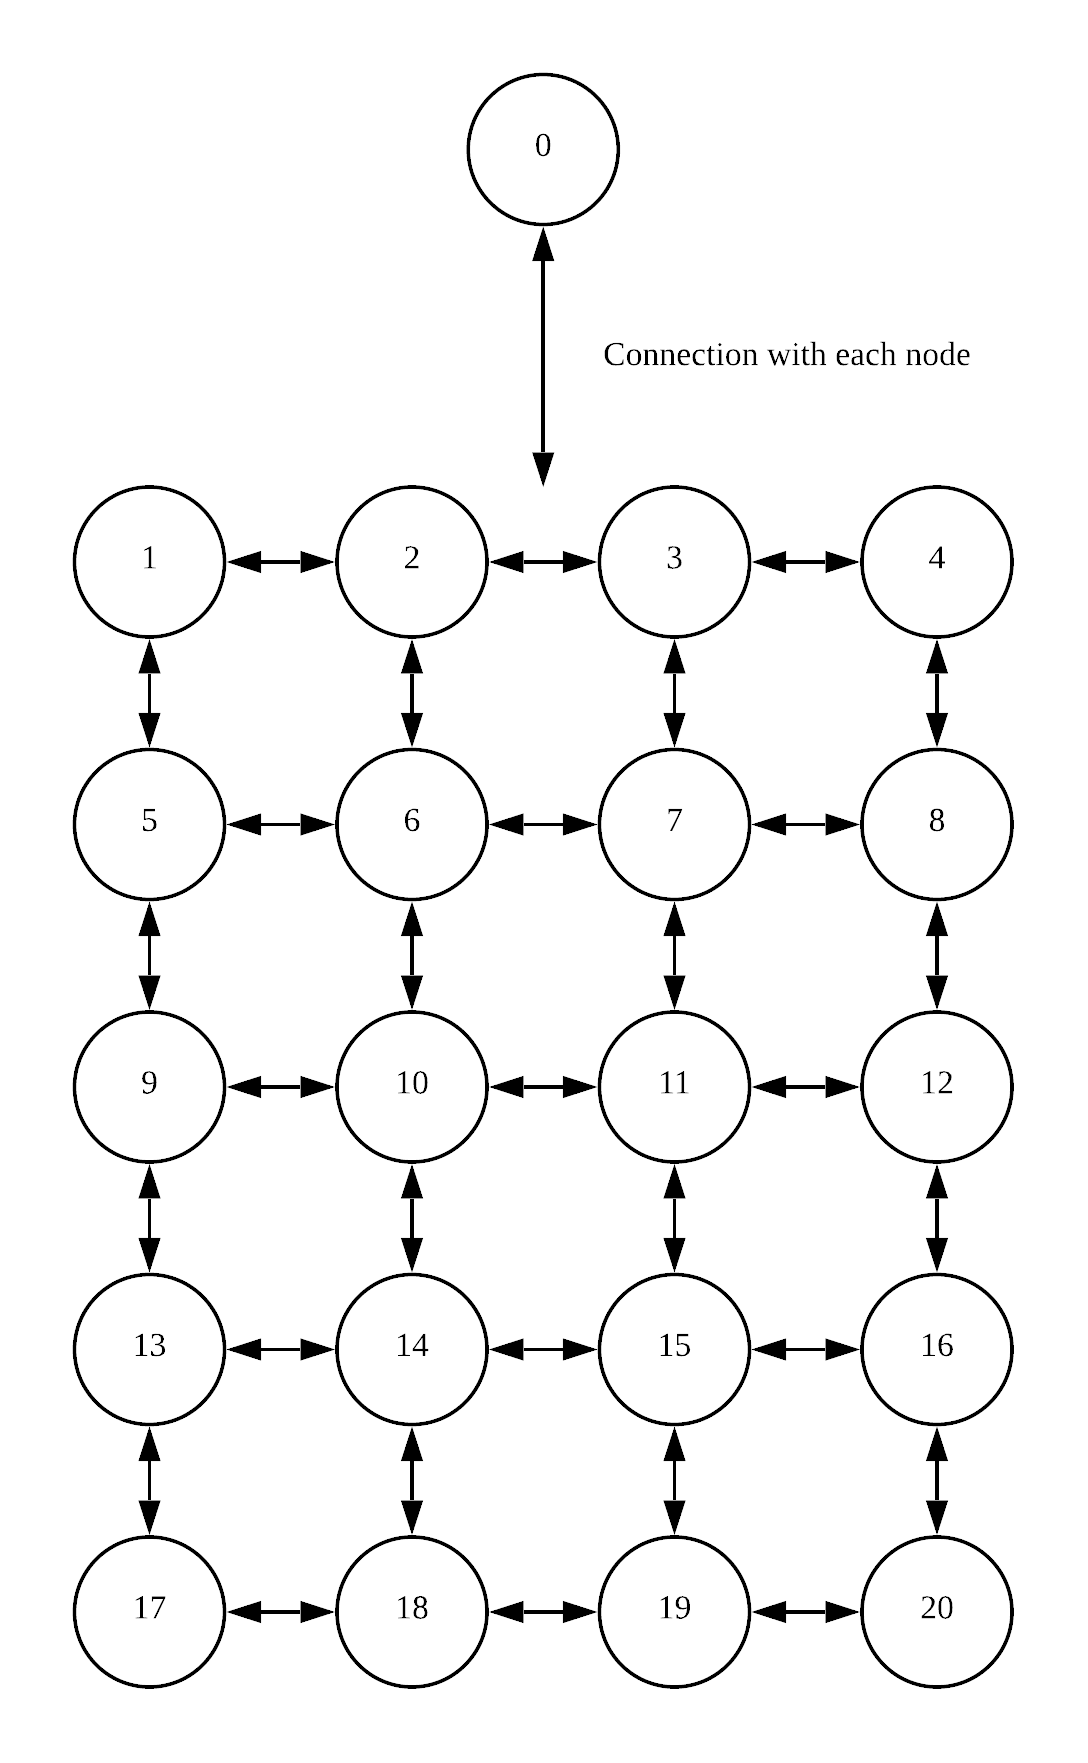
\includegraphics[width=2in]{grid1}
			\label{gridlay1}
		}
		\\
		\subfloat[10 X 2 grid]
		{
			\centering
			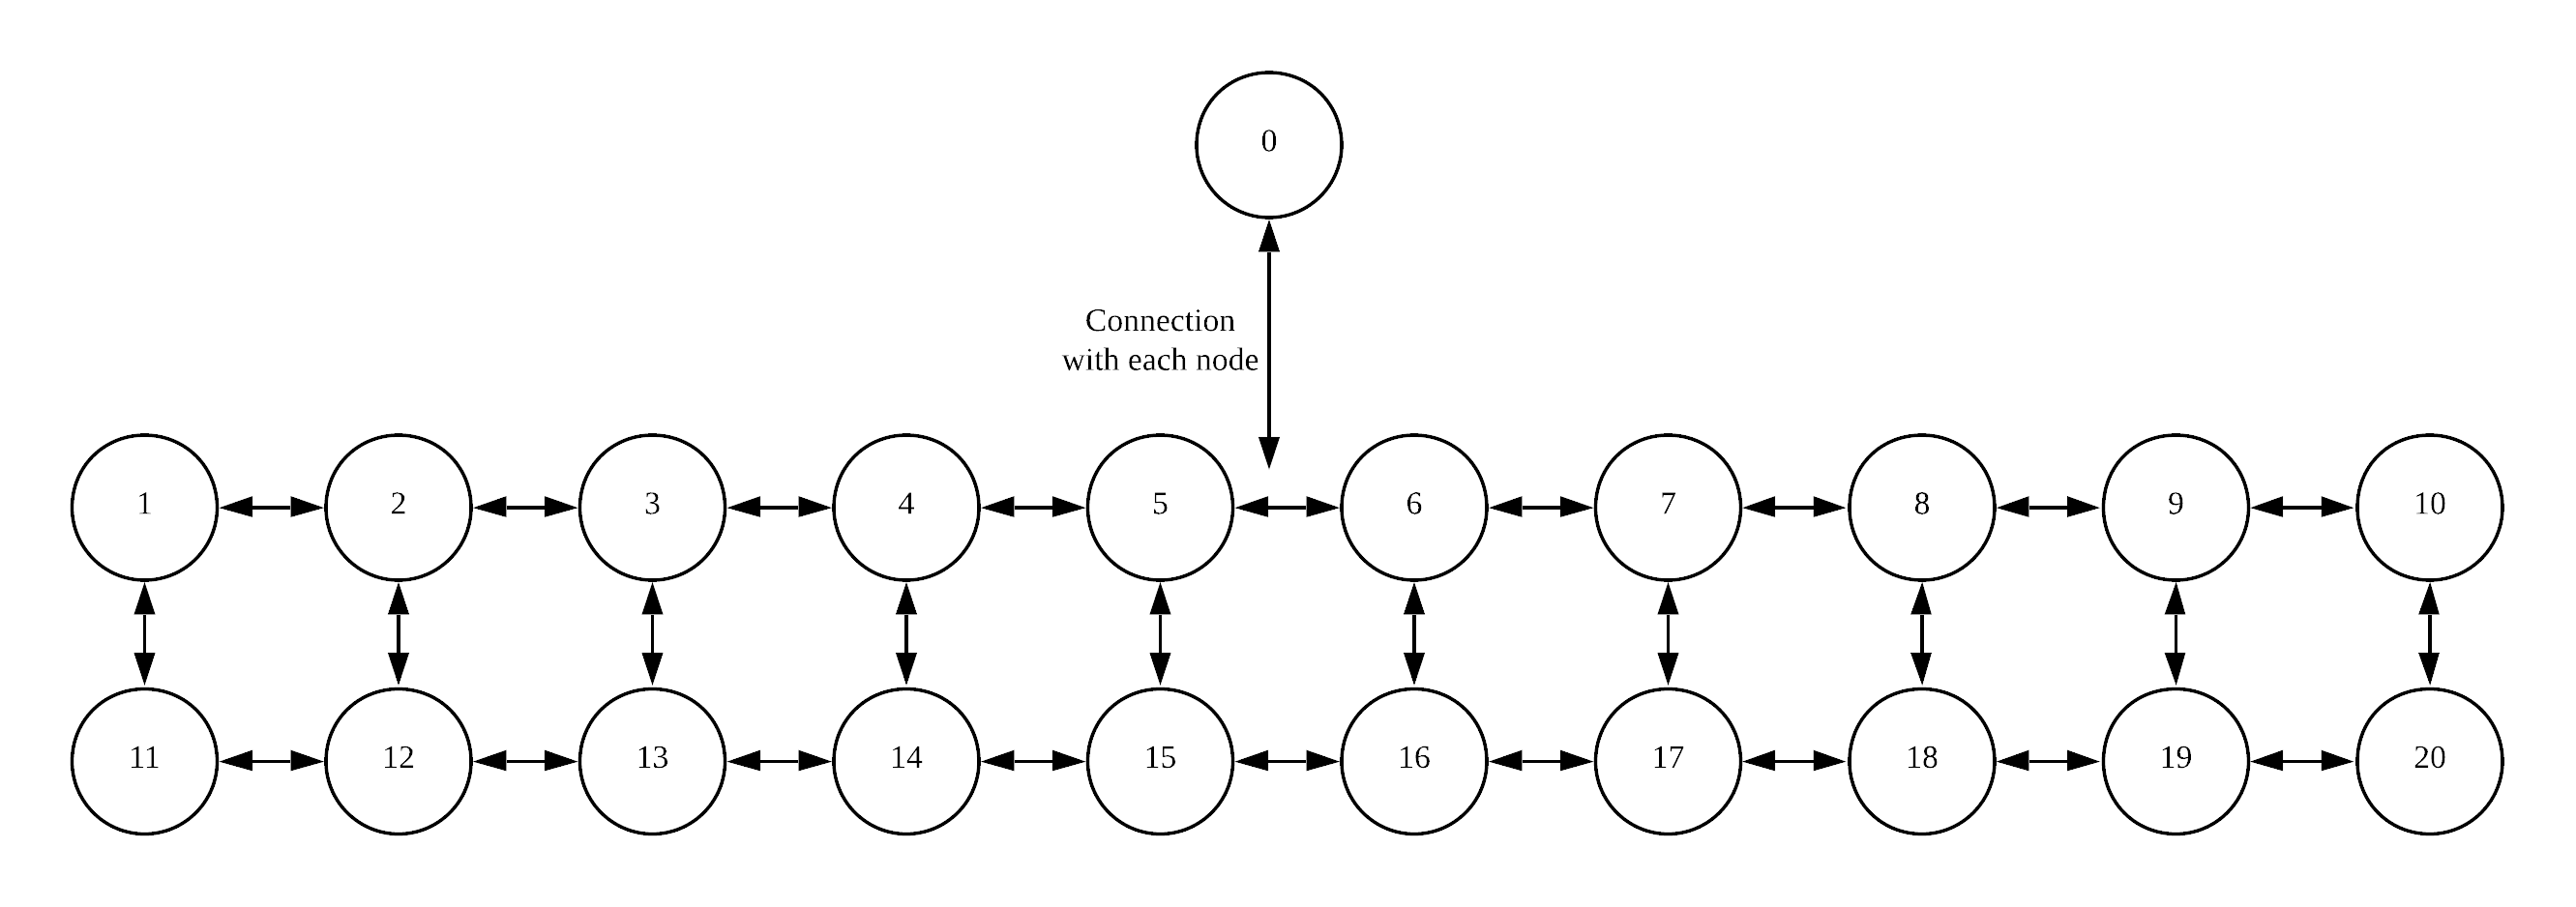
\includegraphics[width=6in]{grid2}
			\label{gridlay2}
		}
		\label{gridlay}
	\end{figure*}
	
	
	After initializing, each node is able to communicate with the adjacent four nodes i.e left, right, top and bottom nodes and also with the base station. The base station is able to communicate with each node individually. The adjacent nodes of each of the sensor nodes are calculated using the height and width specified by the user. Equation \ref{row} and \ref{col} can be used to determine the row index and column index of a given node in the given sensor network. \emph{Do note that we first minus 1 from the current rank, this is due to our base station being rank 0.}
	
	
	\begin{equation}
	row index = (\text{rank} - 1) \quad // \quad \text{width}
	\label{row}
	\end{equation}
	
	
	\begin{equation}
	column index = (\text{rank} - 1) \quad mod \quad \text{width}
	\label{col}
	\end{equation}
	
	After determining the row index and the column index, we can use Equations \ref{left}, \ref{right}, \ref{top} and \ref{bottom} are used to get the four adjacent nodes. \emph{Do note that the shift in the ranks due to base station is in rank 0 is accounted for.}
	
	
	\begin{equation}
	\text{\emph{left}} = row index \times WIDTH + column index
	\label{left}
	\end{equation}
	
	
	\begin{equation}
	\text{\emph{right}} = row index\times WIDTH + column index + 2
	\label{right}
	\end{equation}
	
		\begin{equation}
	\text{\emph{top}} = (row index - 1) \times WIDTH + column index + 1
	\label{top}
	\end{equation}
	
	
	\begin{equation}
	\text{\emph{bottom}} = (row index + 1) \times WIDTH + column index + 1
	\label{bottom}
	\end{equation}
	
	
	Using this process, we do not need to send the rank values to the base station when an event occur. The base station can use the rank of the incoming node to generate the four adjacent nodes in order. 
	

	Published papers..
	
	
	
	
	\subsection{ Encryption/Decryption and its Effects }\label{encryption}
	
	Due to the increase risk of cyber attacks, all wireless networks needs to be encypted as its is easier to attack and steal unencypted data. So, all the messages are encrypted throughout the wireless sensor network. After comparing multiple encryption standards, Advanced Encryption Standard (AES) was used to encrypt the messages.
	
	AES is a symmetric block cipher which can encrypt and decrypt information. Encryption part converts data into cipher text form while decryption part converts cipher text into text form of data.  AES used different 128/192/256 bit keys to encrypt and decrypt data. For the WSN implementation we will be using AES 192, which uses a 192bit key. Since AES is the current standard for wireless communication, financial transactions and e-business we will be using it instead of other encryption algorithms \ref{}. AES has many modes of operations. Examples for these are Electronic Codebook (ECB), Cipher Block Chaining (CBC), Propagating CBC (PCBC), Cipher Feedback (CFB), Output Feedback (OFB) and Counter (CTR).
	
	
	For the WSN, we will be using an online implementation by kokke (ref), which use the Counter (CTR) mode. In order to improve the speed of the encryption process we will be using OpenMP to parallelize the process. The speed up analysis for the encryption algorithm is discussed in Section \ref{encry}.
	
	
	\subsection{ Wireless Sensor Network Event Detection Algorithm }
	
	
	Now we look into the algorithm used by the system to detect events in the WSN. The system is divided into two main sections.
	
	\begin{itemize}
		\item Base Station which logs all the events
		\item Sensor Nodes which triggers and checks for events
	\end{itemize}

	Initially the system generates sensor network grid dynamically using the \emph{width} and \emph{height} given by the user. This was discussed in Section \ref{IPCArc}. Then both the sensor nodes and the base station start running their specific methods. First the IP Address and the MAC Address is sent from each node to be stored in the base station for logging purposes. These messages are encrypted using the AES encryption algorithm discussed in section \ref{encryption}. The base station will then decrypt the message and store it in a dynamic array. Below is the data passed from the node to the base station.
	
		\begin{itemize}
		\item IP Address of the node
		\item MAC Address of the node
	\end{itemize}
	
	Now let us look into the algorithm used by the sensor nodes to generate and detect events.
	
	\subsubsection{Sensor Nodes}
	
	Firstly, each node generates a random number and sends it to the adjacent nodes. This message which contains the random number, sent between the nodes are also encrypted. Then the sensor node starts receiving random numbers from the adjacent nodes. If three or more random numbers are the same, an event is detected. The algorithm also takes into account the random numbers generated by the nodes in the previous iteration. So it works as a sliding window with a time frame depth of 2. Then the nodes will notify the base station by sending a message. This message contains the following details:
	
		\begin{itemize}
		\item The random number that triggered the event
		\item An array of four elements which corresponds to the iteration of the matched value. If the left adjacent node matched with the random number of the previous iteration, the array will contain the iteration number of the previous element in the $0^{th}$ index of the array. 
		\item The MPI Wtime of the event detection to be used to calculate the communication time
		\item The date time string of the time when the event was detected to be used for logging
	\end{itemize}
	
	After sending the message to the server, it saves the random numbers from the current iteration. 
	

	\subsubsection{Base Station}
	After the WSN is initialized, the base station starts checking for messages from any node. If the user has entered -1 as input for the iteration, the system will terminate checking for events only if user enters the keyword "stop". In order for this to work, the base station creates a POSIX thread, which enables it to check for user inputs as well log the events from the nodes. When the user inputs the keyword "stop", the thread then sends a message to the nodes to stop event detection gracefully. 
	
	
		
		
	

	\begin{figure*}[ht]
		\centering
		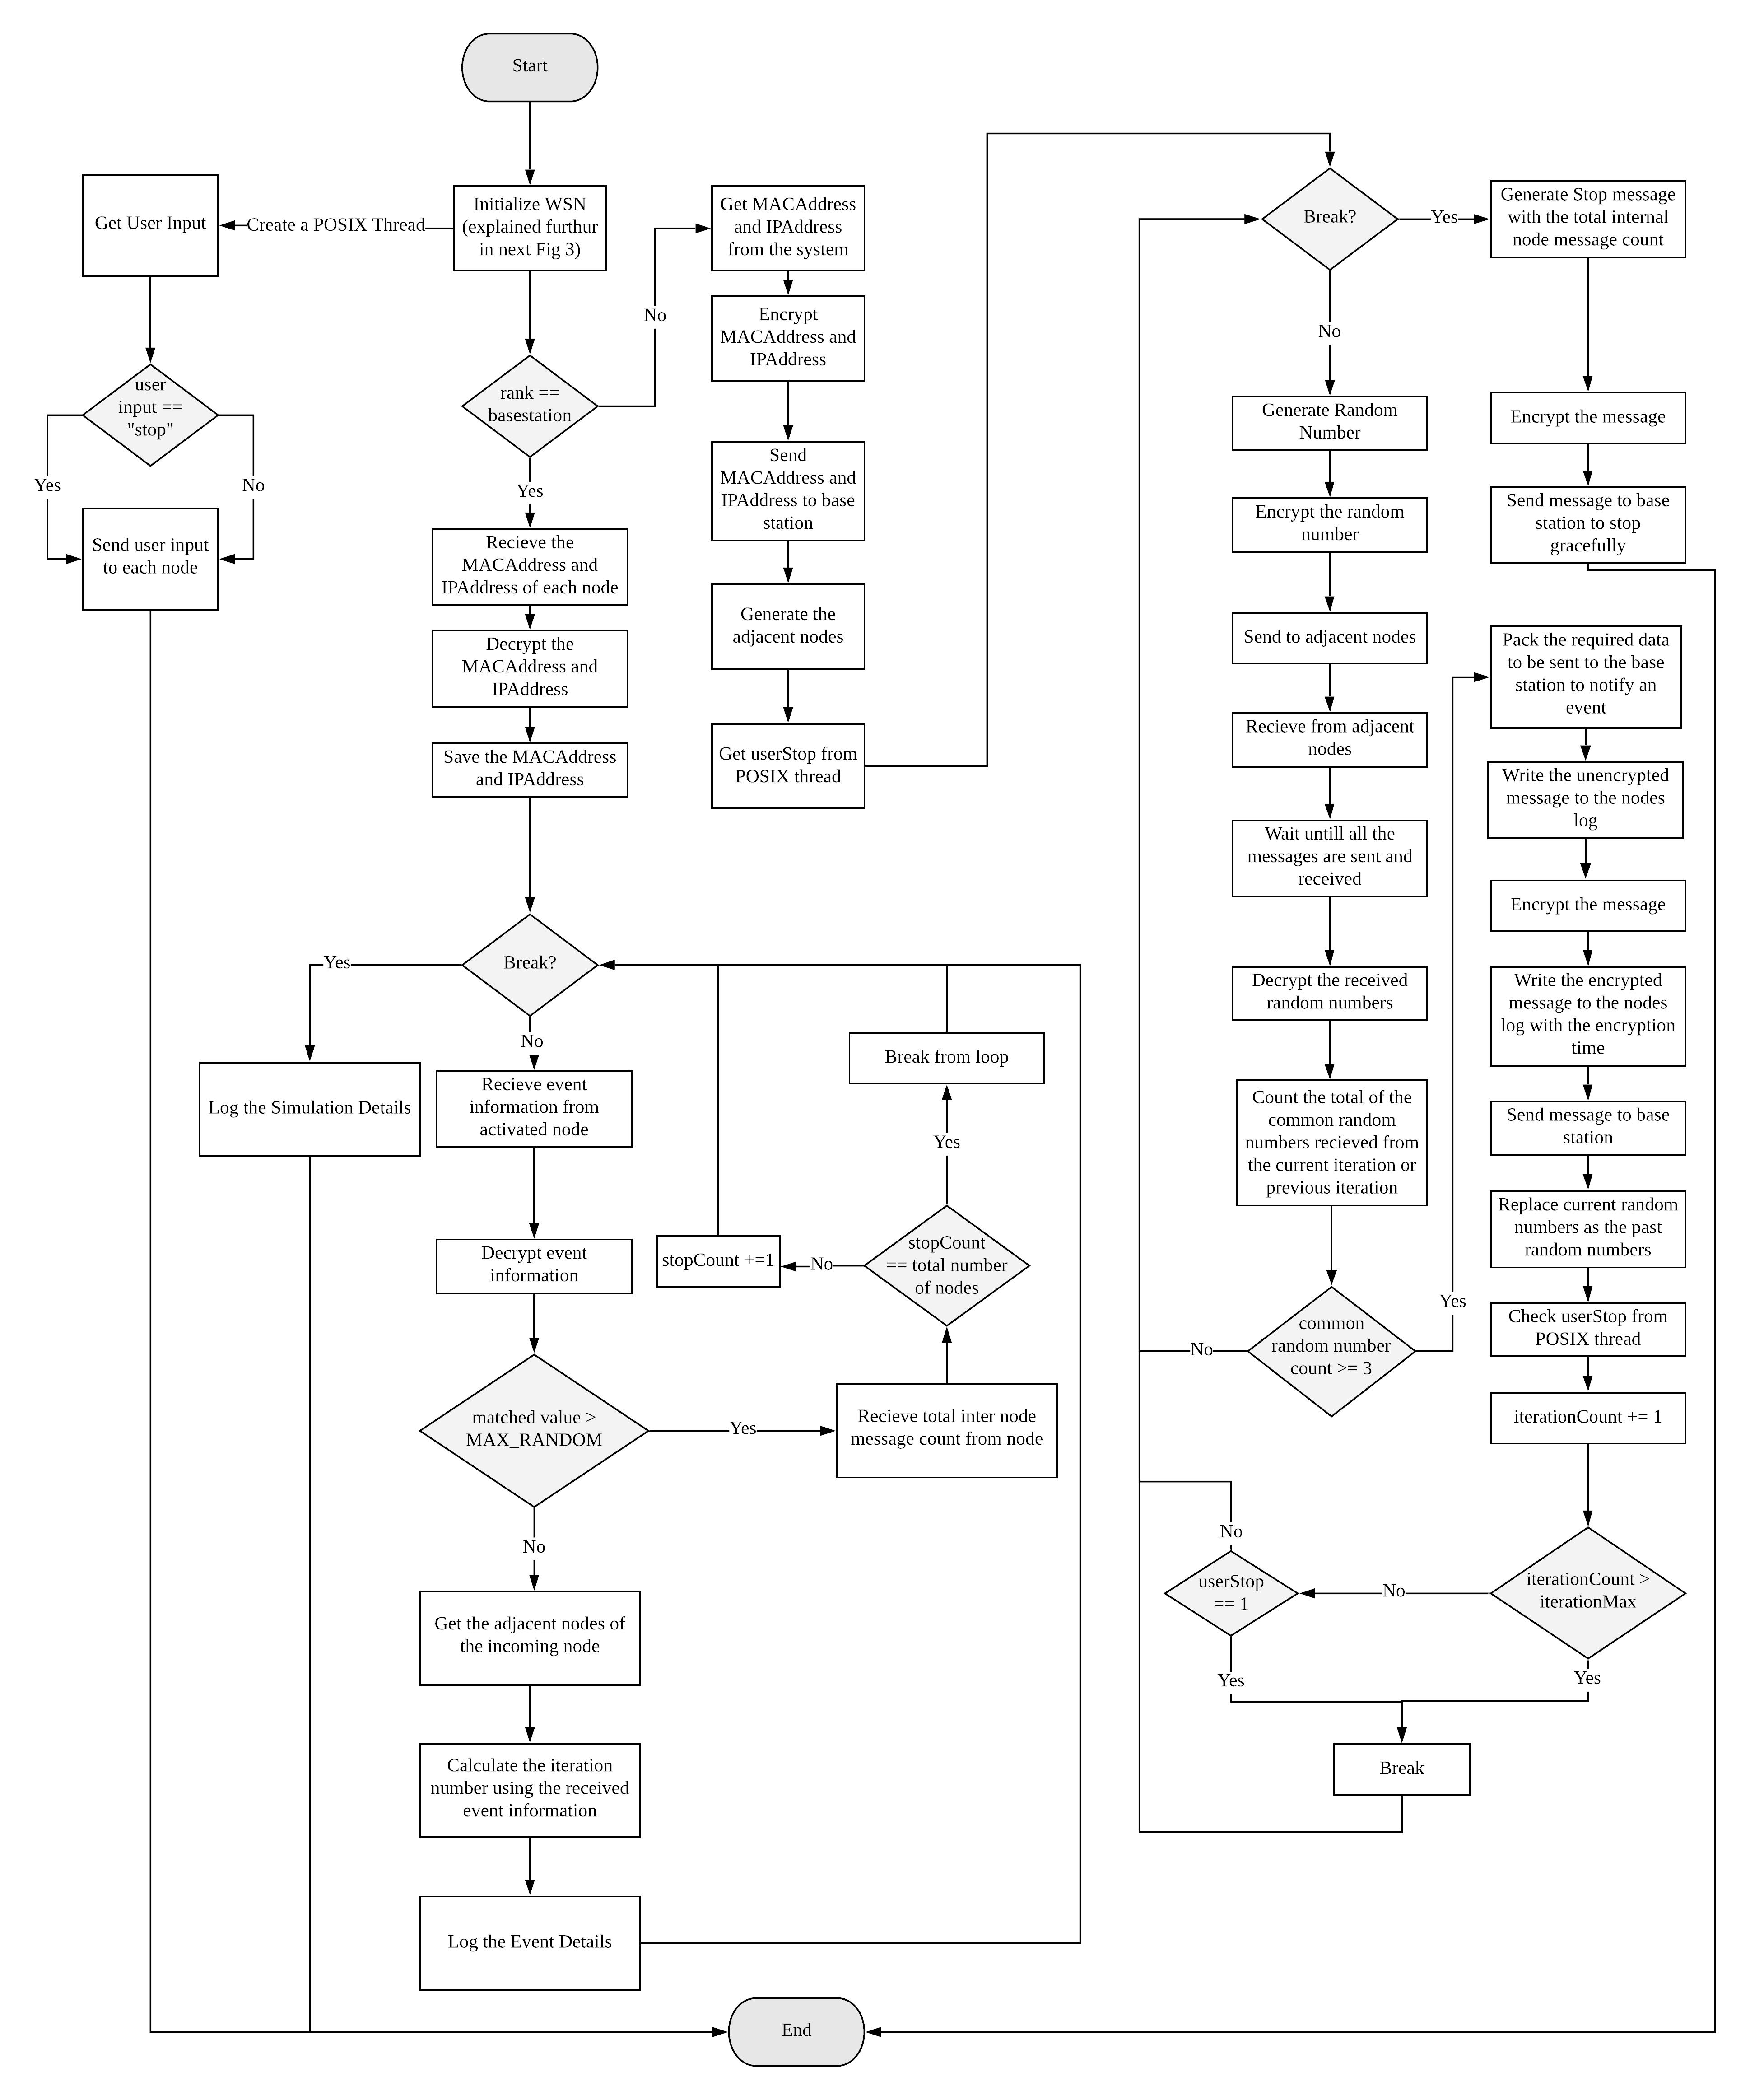
\includegraphics[width=7in]{arc}
		\caption{Technical Flowchart for WSN Inter Process Communication}
		\label{arc}
	\end{figure*}

	\begin{figure}[ht]
	\centering
	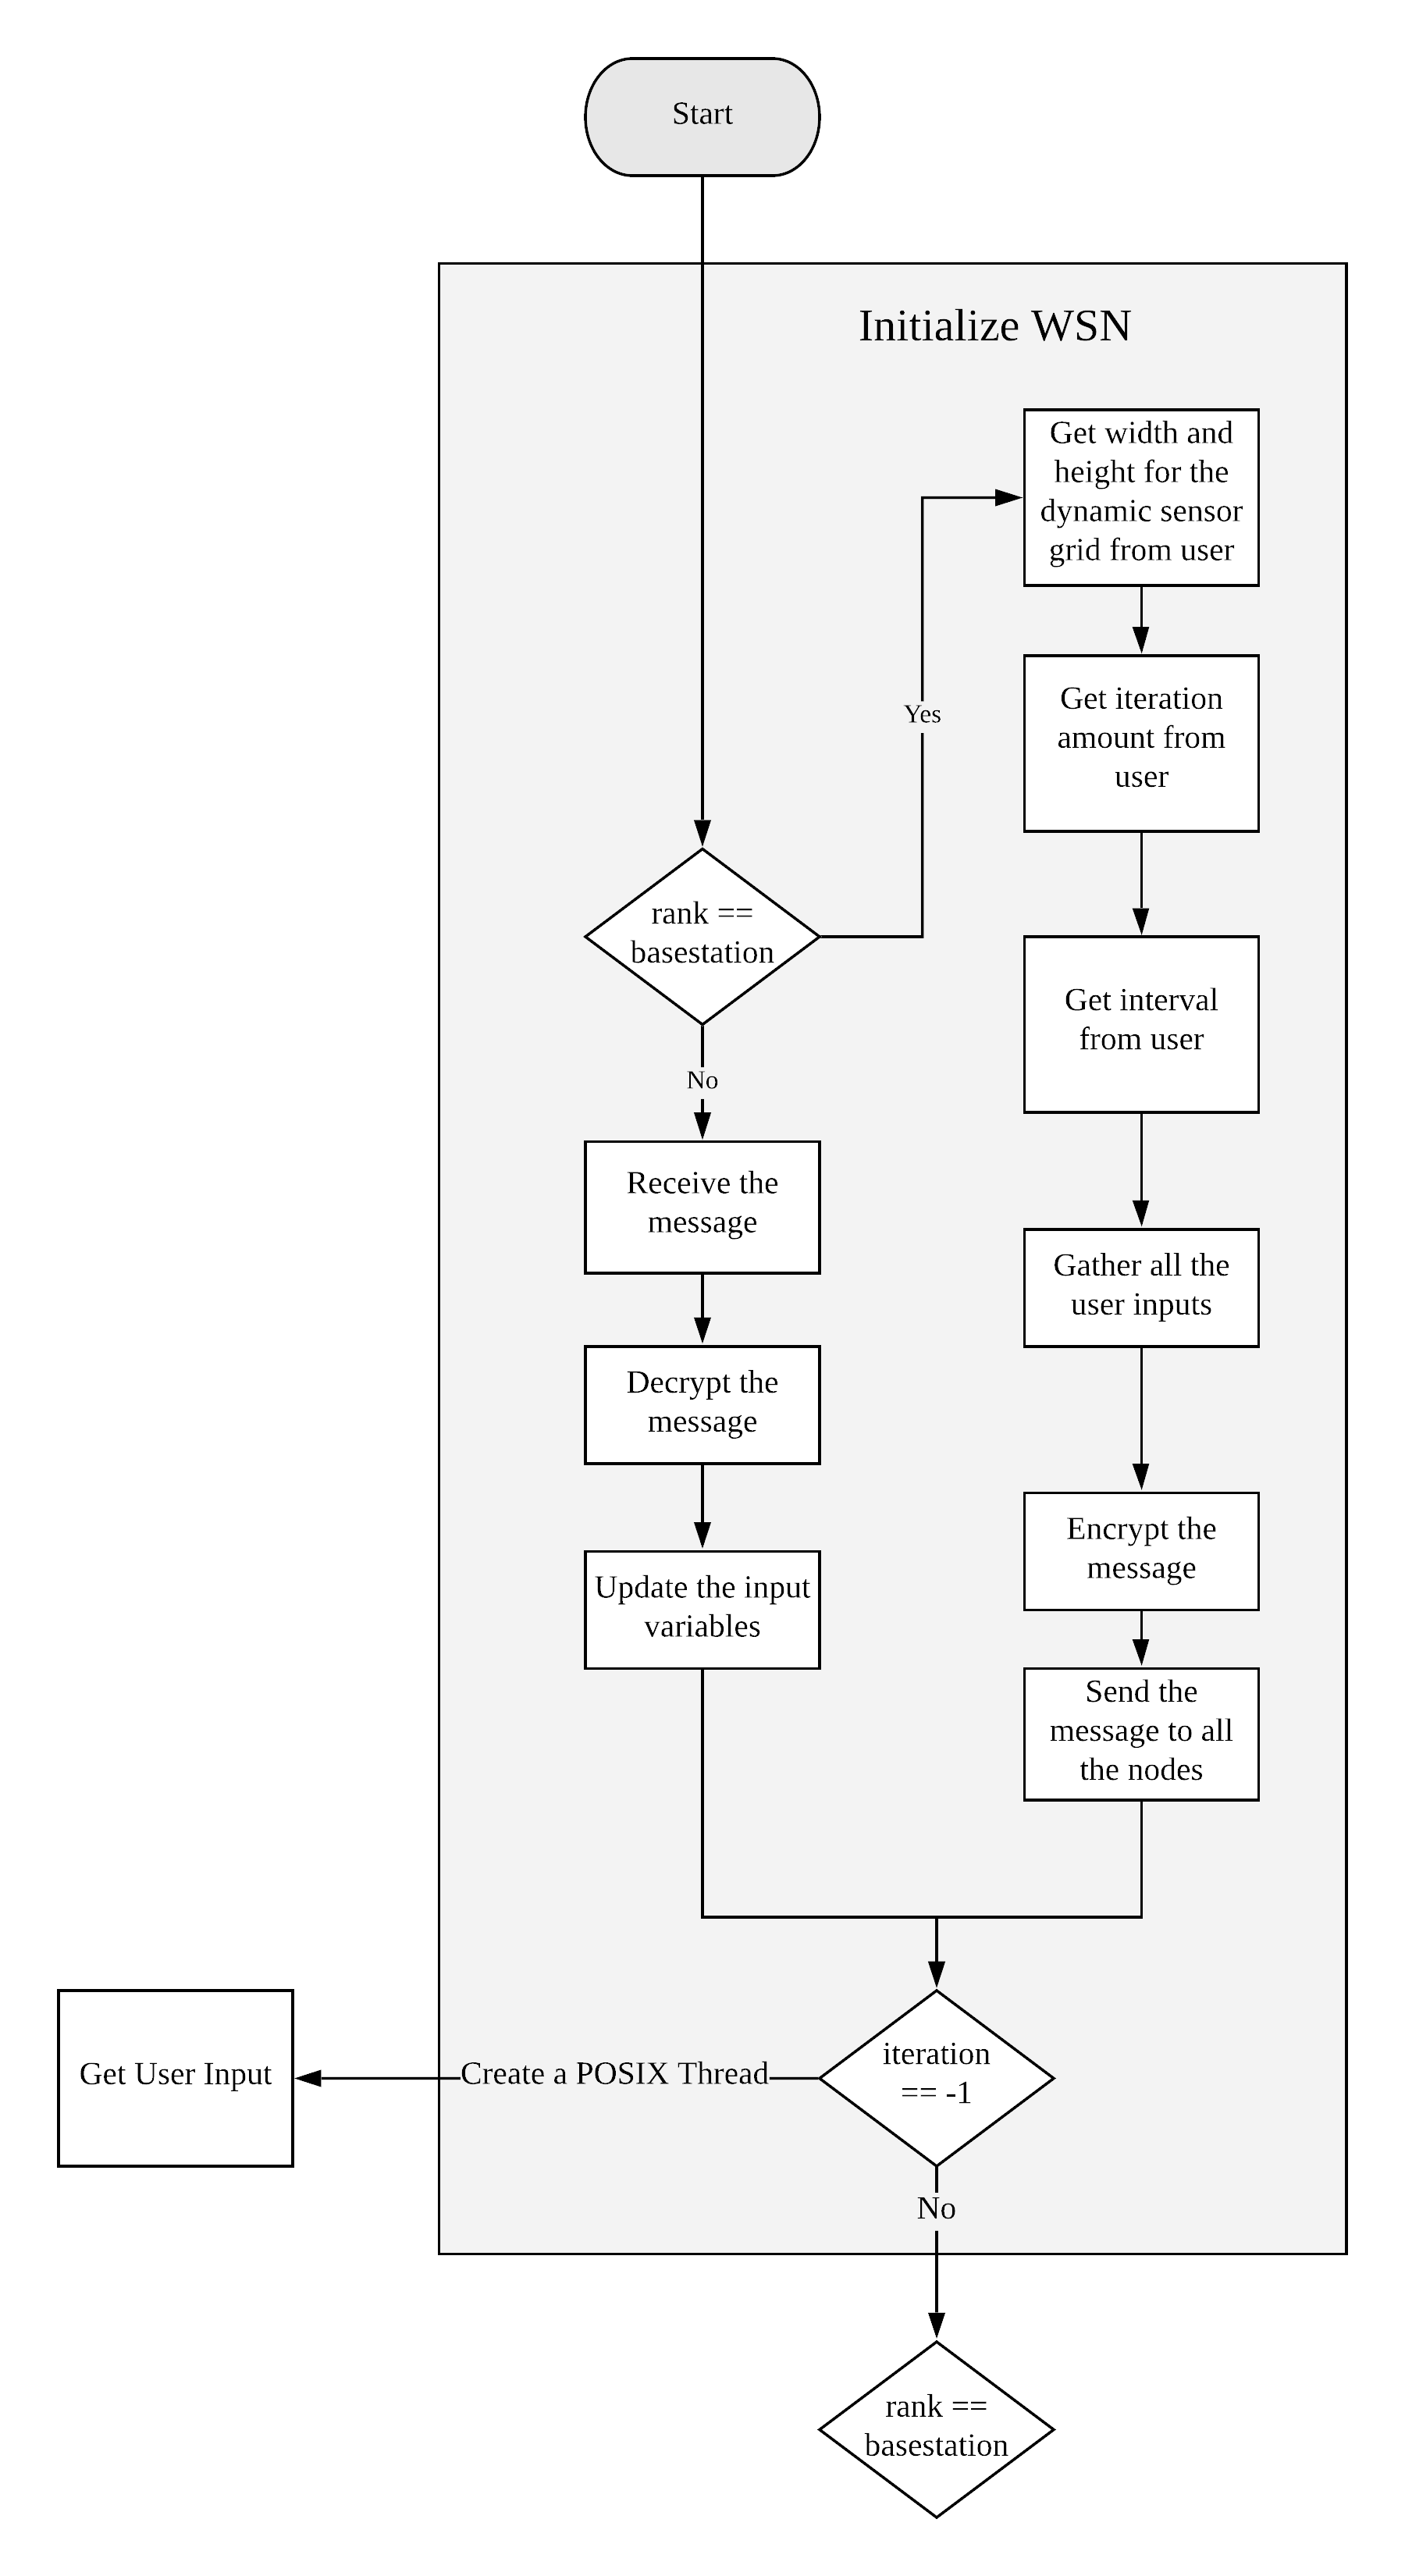
\includegraphics[width=3in]{inWSN}
	\caption{Technical Flowchart for Initializing the WSN}
	\label{inWSN}
\end{figure}
	
	


	
	flow chart for encryption and decryption
	

	\section{Methodology}\label{method}

	In this section we look into the methodology used to test and analyze both the event detection criteria as well as the encryption algorithm used in the WSN. Table \ref{params} summaries the parameters used by the program to get the data required for analysis. The buffer size of the messages used for testing the encryption is different from the actual buffer size which was used to get the results. The reason for this is the smaller buffer size is insignificant to see any speed up when parallelizing the code as they are in milliseconds. So for the encryption test case we used a buffer size of 160000, and for the WSN normal usage test case it was set to 320. 
	
	All of the test cases were run on a 2016 MacBook Pro with an Intel 6820HQ processor, which contains 4 cores and 8 logical cores. Figure \ref{screen 1} in the Appendix shows the screen shot of the console. Another approach for the test case would be to use the dynamic stopping approach. Figure \ref{screen 2} in the Appendix shows the screen shot of the console for this approach.
		
	\begin{table}[!h]\caption{Parameters used for generating the data to be analyzed}
		\begin{center}
			\renewcommand{\arraystretch}{1.2}
			\begin{tabular}{| c | c | c |} 
				\hline
				\textbf{Parameter} & \textbf{Value} & \textbf{Description} \\ \hline
				\emph{Width}    &  4   & \makecell{The width of the sensor \\ node grid }   \\ \hline
				\emph{Height}    &  5   & \makecell{The height of the sensor \\ node grid }   \\ \hline
				\emph{iterations}    &  100   & \makecell{Total number of iteration \\ performed by the system }   \\ \hline
				\emph{interval}    &  1   & \makecell{Wait time between \\ each iteration }   \\ \hline
				\emph{MAXRANDOM}    &  4   & \makecell{Limit the random numbers \\ generated to between 0 - 3 }   \\ \hline
				\emph{packsize}    &  320 and 160000   & \makecell{Size of the buffer for sending\\ and receiving data }   \\ \hline
			\end{tabular}
			\label{params}
		\end{center}
	\end{table}

	\section{Results and Discussion}
	
	This section analyses the results obtained using the methodology described in Section \ref{method}. The analysis is broken down into three main sub sections, each explaining the different aspect of the result.
	
	\subsection{Summary of Events}
	
	When an event is triggered by the sensor, the system generates two types of log files.

	\begin{itemize}
		\item Base Station generates the main log file which logs the event information and the simulation information
		\item Each sensor node logs the the original message, encrypted message and the encryption time
	\end{itemize}

	\subsubsection{Base Station Log File}
	
	The base station logs two types of information, the event detection details and the simulation details at the end. First lets look into the log file to understand each part of it. 
	
	Listing \ref{lst:log} shows an event triggered at the 98 iteration of our test. This can be observed from the first line of the log which determines the iteration number. The next two lines of the logs displays the time when the event was logged on the file and the actual time when the event is detected respectively. This is useful when the node and base station is present in two geographical locations and the time to send the message effects the logging time. But in this example, since the node is a process inside the same machine, we are not able to see a difference. The next two lines denote the node that was triggered i.e. the node that sent the message to the base station.
	
	\begin{lstlisting}[caption={Base station log file},label={lst:log},language=Python]
	--------------------------------------------
	Iteration : 98
	Logged Time : 					Mon 2019-10-14 10:49:21
	Event Occured Time : 		Mon 2019-10-14 10:49:21
	
	Activated Node
	10		78:4f:43:5b:c2:c3		10.156.12.253
	
	Adjacent Nodes
	9			78:4f:43:5b:c2:c3		10.156.12.253		98
	11		78:4f:43:5b:c2:c3		10.156.12.253		97
	14		78:4f:43:5b:c2:c3		10.156.12.253		98
	
	
	Triggered Value : 3
	Communication Time (seconds) : 0.000409
	Decryption Time (seconds) : 0.000048
	Total Messages with server: 451
	Total Activations per Message: 3
	Total Activations : 1371
	--------------------------------------------
	\end{lstlisting}
	
	

	

	


	\subsection{Inter Process Communication Analysis}
	
	charts here
	node diagram here

	\subsection{Encryption Analysis}	\label{encry}
	
	explain speed up here
	check byte log files
	
	

	\section{Conclusion}
	
	\section{Future Work}
	

	
\bibliographystyle{IEEEtran}
\bibliography{ref.bib}

	\newpage
	\onecolumn
	\appendix
	
	
\begin{figure*}[h]
	\centering
	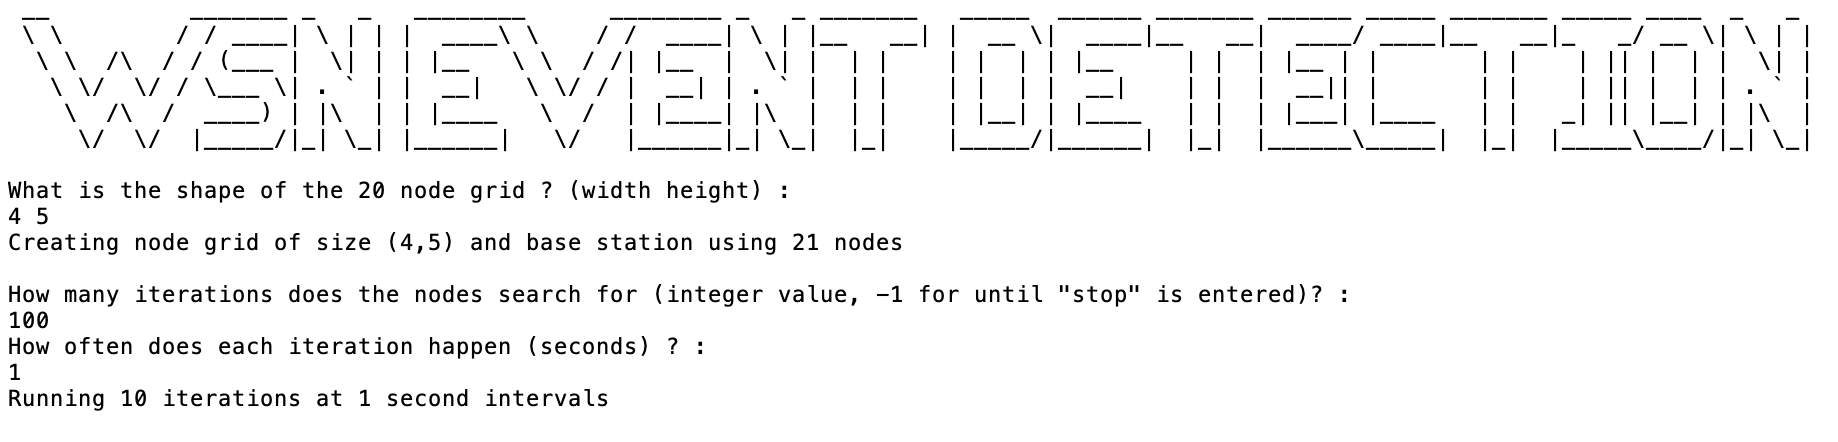
\includegraphics[width=6in,keepaspectratio]{console1}
	\caption{Screenshot of the console used for the generating the results}
	\label{screen 1}
\end{figure*}

\begin{figure*}[h]
	\centering
	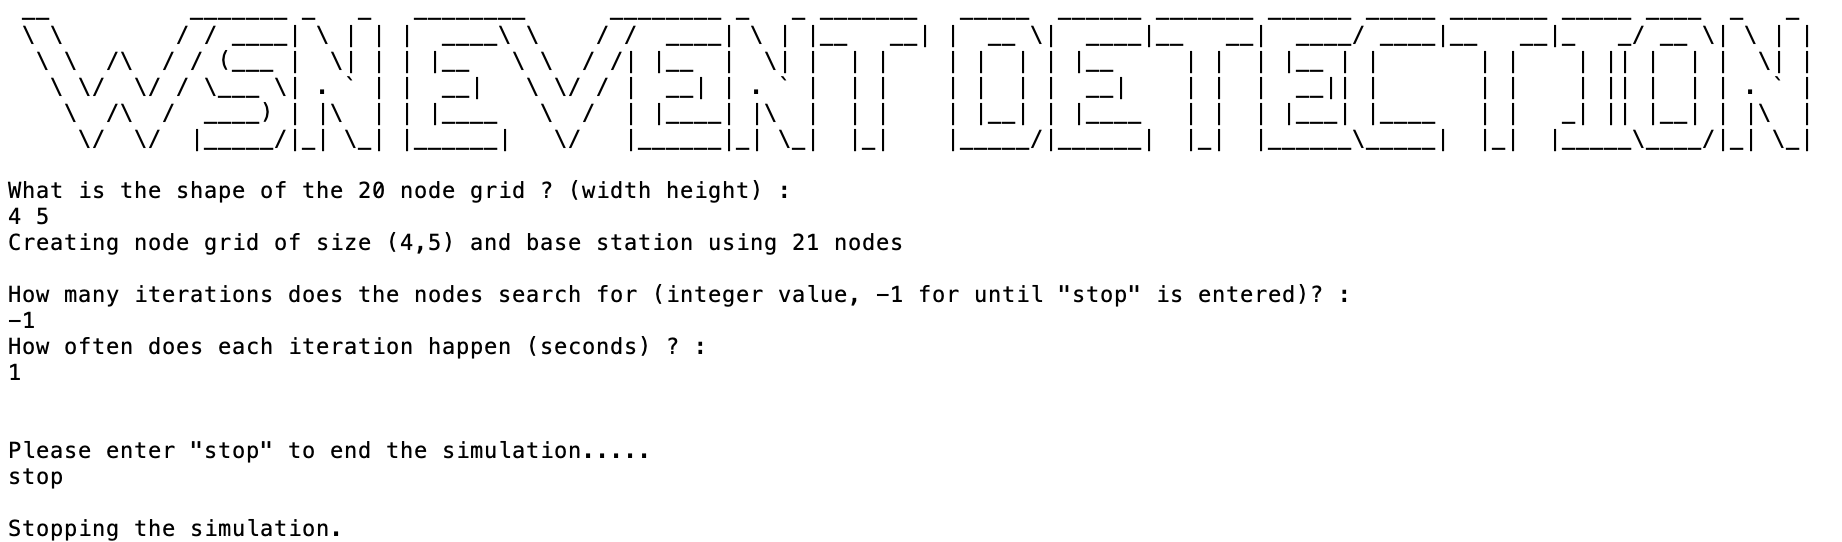
\includegraphics[width=6in,keepaspectratio]{console2}
	\caption{Screenshot of the alternative approach to run the program until user enters stop}
	\label{screen 2}
\end{figure*}

\end{document}
